
\section{Hardware}
\label{Sec:5-hardware}
\subsection{Raspberry - Sistema Operacional}
\paragraph{
	Raspberry Pi é um computador, como tal é possível usá-lo sobre um sistema operacional. O sistema operacional usado é o Raspian, um sistema operacional baseado no Debian customizado para rodar no raspberry pi. Apesar de, teóricamente, não ser necessário o raspberry usar um sistema operacional, facilita muito o desenvolvimento tal equipamento conter uma interface amigávelpara seu uso.
}
\subsection{Raspberry - Adaptador Wifi}
\paragraph{
	Após o sistema Raspian ser instalado no cartão de memória, foi necessário configurar o adaptador Wifi. O modelo usado é o TP-Link TL-WN723N.
}

\subsubsection{Procedimentos}
\begin{lstlisting}
wget https://dl.dropboxusercontent.com/u/80256631/8188eu-3.18.11-v7-781.tar.gz
tar xzf 8188eu-3.18.11-v7-781.tar.gz
./install.sh
\end{lstlisting}

\begin{figure}[H]
\centering
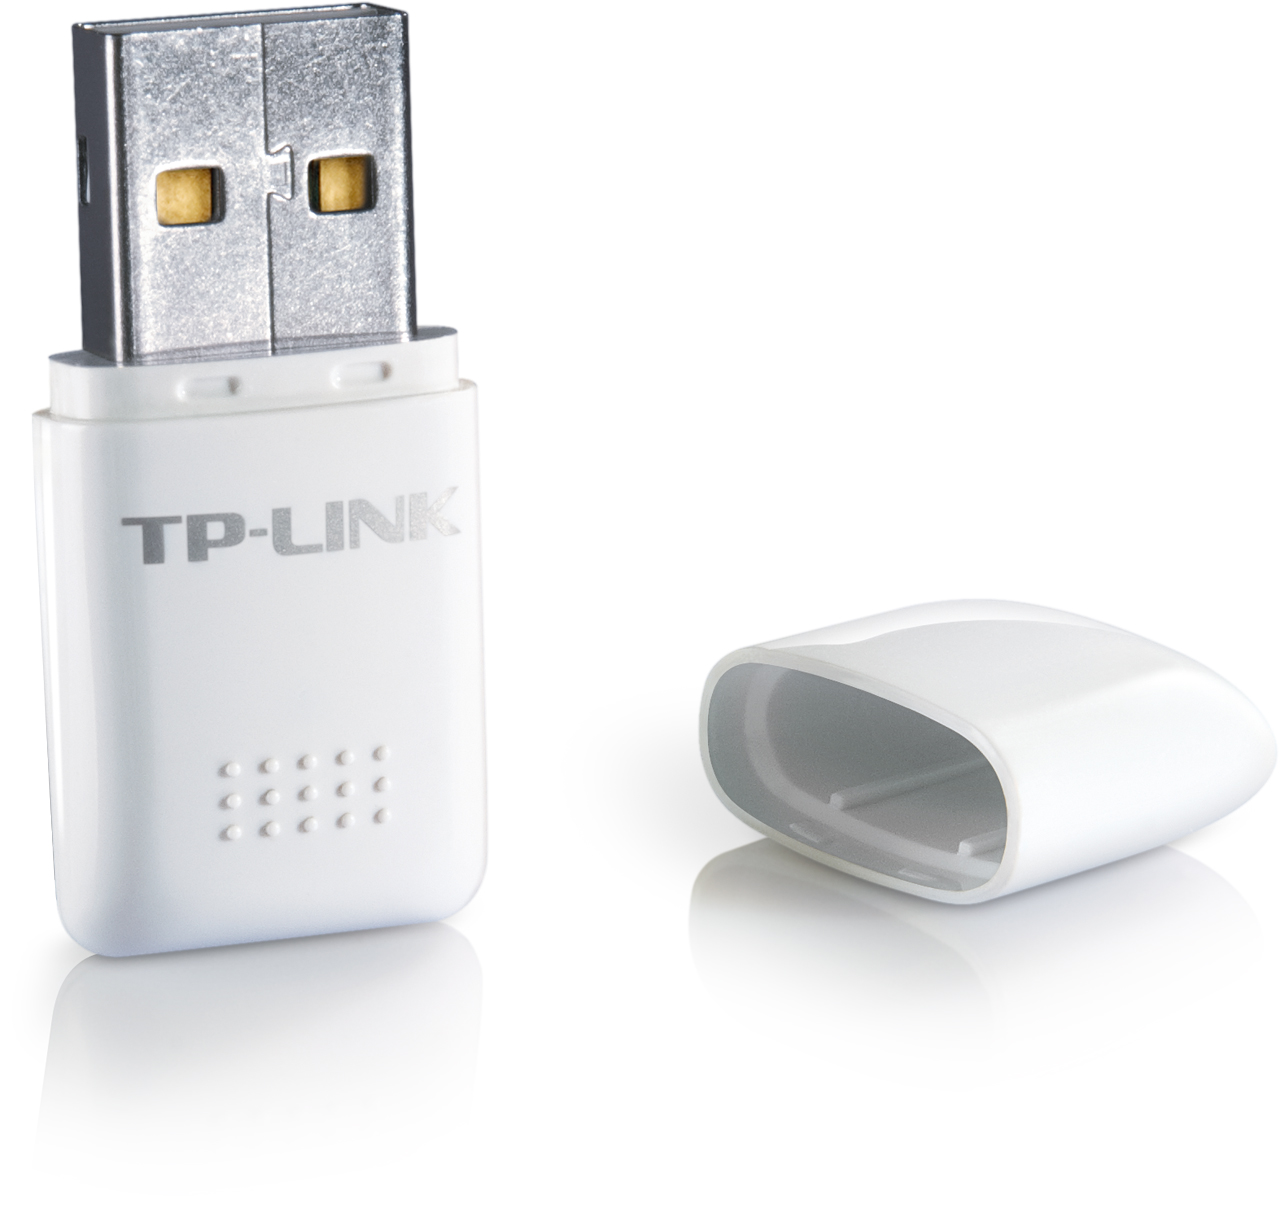
\includegraphics[width=5cm,height=5cm,keepaspectratio]{figuras/wifi-adapter.jpg}
\caption{\label{fig:wifi-adapter} Adaptador wifi usado no raspberry}
\end{figure}
